\newpage
\subsection{Dams}
A dam is a large, man-made structure built to contain some body of water. In addition to construction for the purpose of producing hydroelectric power, dams are created to control river flow and regulate flooding.

In October of 2010, a report has been made on the strategic environmental assessment of hydroelectric power on the Mekong mainstream by the Mekong River Commission.\cite{mrc} The report generally concluded to limit the amount of mainstream dams. While this report was published over 10 year ago, it is useful to take a closer look at it to see the current dam issues at hand.

\subsubsection{The benefits of dams}
Hydroelectric energy generated by dams are by far the most prevalent renewable energy source in the world, and will continue to be a key energy source in the future as countries move away from coal, natural gas, and oil.

Dams also allow one to control floodwaters and supply a fixed amount of fluid to areas for controlled irrigation. On a local level, dams have the unique ability to optimize a river for both energy delivery and agricultural irrigation.

\subsubsection{\textit{Regional differences}}
While locally there might be many benefits for implementing dams, the ability to control the flow of the water leads to a slew of issues. Downstream farmers for example in countries such as Vietnam and Cambodia depend on the Mekong floods for their irrigation, and are very dependent on other parties if the water is artificially controlled upstream. 

\begin{figure}[h]
\centering
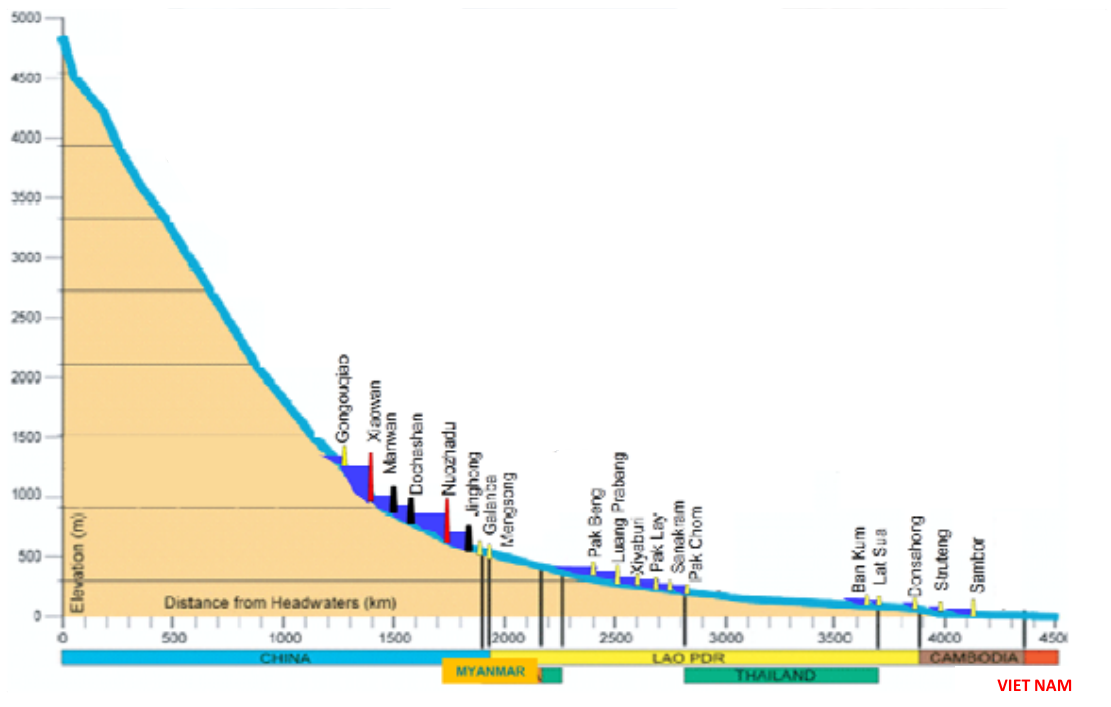
\includegraphics[scale=0.55]{mekong/11_proposed.png}
\caption{Mekong mainstream hydropower projects \cite{mrc}}
\end{figure}

Many of the benefits can be seen upstream, while many of the downsides can be seen downstream. This can lead to tensions between countries, as there is effectively a trade of wealth.\\

Lao PDR gains for example most from the overall power benefits directly associated with mainstream hydro power. Mainstream hydro power is less significant for the power sectors of Thailand and Vietnam, where the impact of the electricity prices are minor (less than 1.5\%).

Some downsides of the dams apply to different regions however. As a conservative estimate, the mainstream damming projects are expected to be responsible for one third of the reduction in nutrient and sediment loads of the Mekong River. This can translate into increasing food insecurity in the basin. If natural resources productivity is reduced, the countries most at risk are Cambodia and Lao PDR.

In March of 2010, the Mekong Delta reached its lowest water levels in 50 years. It opened the discussion between countries what effect hydropower dam development has on the Mekong Delta. \cite{globalissues} Looking back today, it seems that those discussions have not helped much. \\

The water levels reached its lowest point again in 2020. Dams are taking water out of the system during the wet season and putting it back in the dry season, resulting in the level of the river being too low for any sort of irrigation throughout the year. According to local farmers, the lower Mekong Delta is now salty for up to four months instead of the usual one month of the year, and entire fields of trees are are being killed by saltwater intrusion. \cite{voanews}



\begin{figure}[h]
\centering
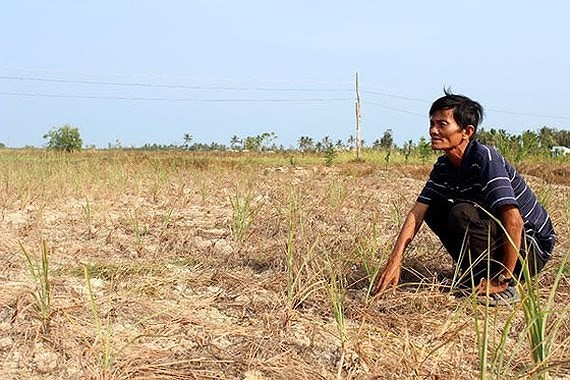
\includegraphics[scale=0.55]{mekong/41_paddy.jpg}
\caption{The drought-stricken Mekong River in Pak Chom district in the northeastern Thai province of Loei. 
\cite{voanews}}
\end{figure}

\subsubsection{Mitigation}
Several strategies have been developed for mitigating issues of the dams. Fish ladders may be a mitigation option for low dams on tributaries, but existing types and sizes of fish ladders cannot accommodate the intensity and diversity of fish migrations on the mainstream. Fishery reservoirs were proposed instead, but they would only be capable of producing 10\% of the lost capture fisheries.

If dams are continued to be used, the irrigation sector needs significant investment to re-equip it for use of reservoir water instead of using water from the Mekong Delta.